% !TEX encoding = UTF-8 Unicode
% !TEX TS-program = pdflatex
%
% Esempi d'uso degli ambienti frontespizio (e frontespizio*)
\documentclass[%
% copo=10pt,10pt
corpo=11pt,
% corpo=12pt,
twoside,
 stile=classica,
oldstyle,
%autoretitolo,
greek,% per comporre parte del testo in greco (qui solo con classica)
%cucitura,
]{toptesi}
% \usepackage{teubner}% per le notazioni filologiche greche
%
%%%%%%%%%%%%%%%%%%%%%%%%%%%%%%%%%%%%%%%%%%%%%%%%%%%%%%%%%%%%
% per macchine Linux/Mac/UNIX/Windows; sarebbe meglio utf8
%\usepackage[latin1]{inputenc}
\usepackage[utf8]{inputenc}
\usepackage[T1]{fontenc}
\usepackage{lmodern}
\usepackage{textcomp}
\usepackage[a-1b]{pdfx}
\usepackage{longtable}
%%%%%%%%%%%%%%%%%%%%%%%%%%%%%%%%%%%%%%%%%%%%%%%%%%%%%%%%%%%%%%%%%
\usepackage{lipsum}% Per scrivere testo fasullo in "latinorum"

\usepackage{pict2e}% elimina ogni limitazione all'ambiente picture
%

%\english%  di default la lingua è impostata con \italiano


\iflanguage{english}{%
	\retrofrontespizio{This work is subject to the Creative Commons Licence}
	\DottoratoIn{PhD Course in\space}
	\CorsoDiLaureaIn{Master degree course in\space}
	\NomeMonografia{Bachelor Degree Final Work}
	\TesiDiLaurea{Master Degree Thesis}
	\NomeDissertazione{PhD Dissertation}
	\InName{in}
	\CandidateName{Candidates}% or Candidate
	\AdvisorName{Supervisors}% or Supervisor
	\TutorName{Tutor}
	\NomeTutoreAziendale{Internship Tutor}
	\CycleName{cycle}
	\NomePrimoTomo{First volume}
	\NomeSecondoTomo{Second Volume}
	\NomeTerzoTomo{Third Volume}
	\NomeQuartoTomo{Fourth Volume}
	\logosede{logouno}% or comma separated list of logos
}{}
%%%%%%%%%%%%%%%%%%%%%%%%%%%%%%%%%%%%%%%%%%%%%%%%%%%%%%%%%%%%%%%%%%%%%%%%%%%%%%%%%%%%%%%%

%%%%%%%%%%%%%%%%%%%%%%%%%%%%%%%%%%%%%%%%%%%%%%%%%%%%%%%%%%%%%%%%%%%%%%%%%%%
% Lasciare questo per ultimo dopo aver caricato tutti gli altri pacchetti
%
% Commentare la riga seguente se si è specificata l'opzione "pdfa"
\usepackage{hyperref}

\hypersetup{%
    pdfpagemode={UseOutlines},
    bookmarksopen,
    pdfstartview={FitH},
    colorlinks,
    linkcolor={blue},
    citecolor={blue},
    urlcolor={blue}
  }
%%%%%%%%%%%%%%%%%%%%%%%%%%%%%%%%%%%%%%%%%%%%%%%%%%%%%%%%%%%%%%%%%%%%%%%%%

%%%%%%% Definizioni locali
\newtheorem{osservazione}{Osservazione}% Standard LaTeX



\begin{document}
\errorcontextlines=9% debugging


%%%%%%%%%%%%%%%%%%%%%%%%%%%%%%%%%%%%%%%%%%%%%%%%%%%%%%%%%%%%%%%%%%%%%%%%%%%%%%%%%%%%%%
% Questo codice serve per collaudare gli ambienti frontespizio e frontespizio*
% con l'asterisco il logo dell'ateneo va a finire sotto il titolo nella seconda
% metà della pagina; senza asterisco va a finire in testa.

\begin{frontespizio}
\ateneo{Politecnico di Torino}% nome generico dell'universita'
%\ateneo{}% nome generico vuoto per sperimentare nei vari casi
\nomeateneo{}% nome proprio dell'universita'
\FacoltaDi{}% prefisso vuoto per la facolta'
\facolta[III]{}% dottrine della facolta'
\titolo{Dimensionamento di un braccio robotico a 6 assi}% per la laurea quinquennale e il dottorato
\sottotitolo{Progetto rover Trinity - Team DIANA}% per la laurea quinquennale e il dottorato
\corsodilaurea{Ingegneria Meccanica}% per la laurea
\renewcommand*\IDlabel{\\\quad matricola: }% per ridefinire il prefisso del numero di matricola
\candidato{Luigi \textsc{Di Rado}}[204427]% per tutti i percorsi
%\secondocandidato{Evangelista \textsc{Torricelli}}[123457]% solo per l. magistrale 
\relatore{prof.\ Stefano Pastorelli}% per la laurea e/o il dottorato
%\secondorelatore{dipl.~ing.~Werner von Braun}% solo per la laurea magistrale
%\tutoreaziendale{dott.\ ing.\ Giovanni Giacosa}
%\NomeTutoreAziendale{Supervisore aziendale\\Centro Ricerche FIAT}
\sedutadilaurea{\textsc{Anno~accademico} 2019-2020}% per la laurea magistrale
\ciclodidottorato{XV}% solo per il dottorato
\logosede{logouno} % questo e' ovviamente facoltativo
\end{frontespizio}
%%%%% 


% \paginavuota % funziona anche senza specificare l'opzione classica

\ringraziamenti % stampa i ringraziamenti, di solito superflui e inutili




\mainmatter
\indici
\chapter{Rover Esplorativi e di Assistenza: Scenari di missione}
Il team DIANA, acronimo di  \textit{Ducti Ingenio Accipimus Naturam Astrorum}, lavora nella ricerca e nello sviluppo della robotica per applicazioni spaziali.
Il Team è stato fondato nel 2008 in occasione del progetto nazionale AMALIA e ha prodotto tre prototipi di rover: \textbf{Amalia}, un rover lunare esplorativo, \textbf{T0-R0}, un rover marziano di assistenza che ha partecipato a European Rover Challenge 2018 e \textbf{TRINITY}, il nuovo rover marziano che ha partecipato all'European Rover Challenge 2019.

\begin{figure}
	\centering
	\begin{tabular}{ll}
		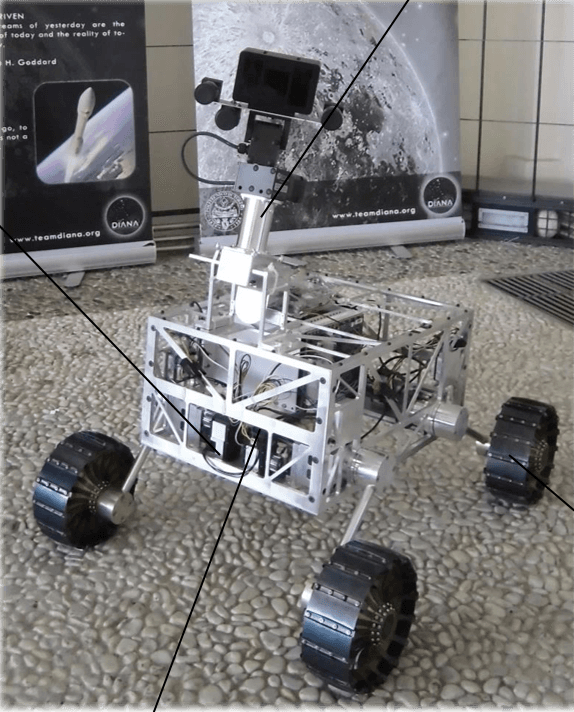
\includegraphics[width=.3\textwidth]{image/amalia.png}
&
		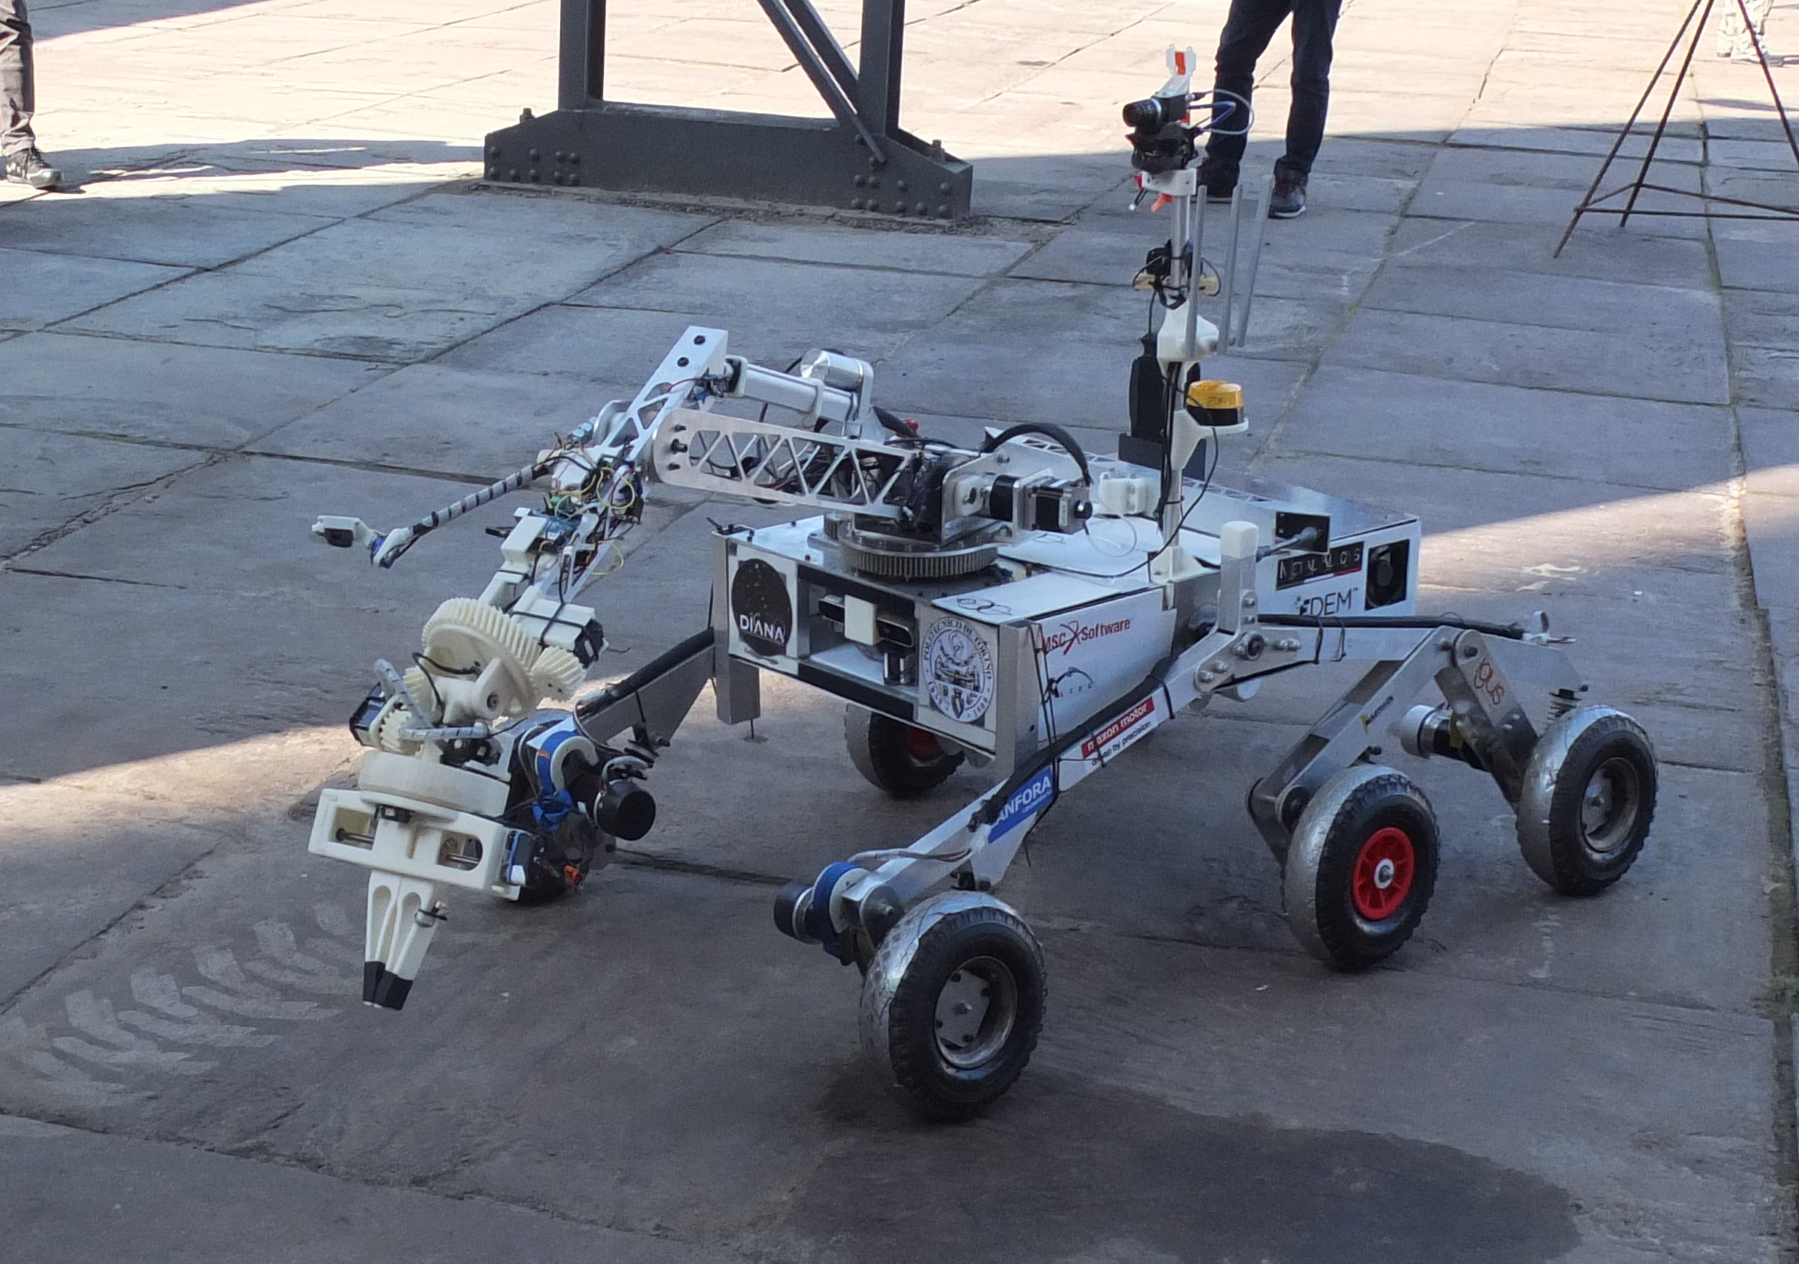
\includegraphics[width=.5\textwidth]{image/toro.jpg}
	\end{tabular}
		\caption{Rover AMALIA E T0-R0}
		\label{fig:amaliatoro}
	
\end{figure}

Il team DIANA ha un'esperienza decennale nella progettazione e nello sviluppo di modelli di rover per l'esplorazione e l'assistenza e dispone di un set completo di abilità ingegneristiche, ottima conoscenza del software ed eccezionali capacità organizzative, gestionali e di lavoro di squadra, tutte cruciali nella produzione di un progetto complesso.
Il team intende porre le basi per un nuovo approccio all'ingegneria aerospaziale, contribuendo a portare la robotica spaziale a un livello più accessibile grazie alla sua tecnica di lavoro innovativa.
TRINITY è il prodotto del patrimonio e della competenza di dieci anni di duro lavoro e ricerca approfondita, condotta con una visione chiara e un approccio specifico.
Il team sta affrontando una crescita dal 2018 e la partecipazione all'European Rover Challenge ha avuto un ruolo chiave nel suo sviluppo poiché rappresenta un'opportunità senza precedenti per testare le soluzioni del team e capire dove e come migliorare il suo progetto.

\begin{figure}
	\centering
	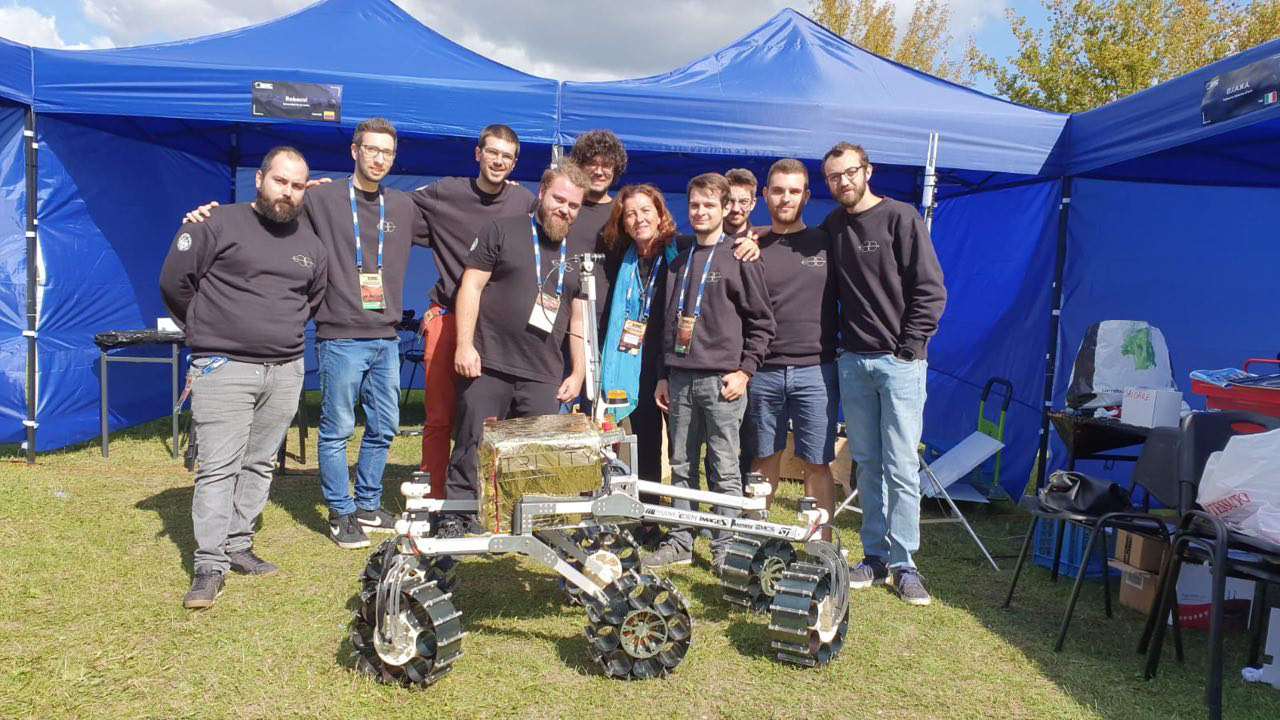
\includegraphics[width=0.6\textwidth]{image/trinityerc.jpeg}
	\caption{Il Team DIANA con TRINITY ad ERC 2019}
	\label{fig:trinityerc}
\end{figure}


Nell'ambito del team DIANA che sta diventando un forte gruppo di giovani ingegneri che lavorano nella ricerca e nello sviluppo della robotica spaziale, testare il lavoro svolto in laboratorio è un passo cruciale nello sviluppo.
Inoltre, il Team DIANA ha vissuto l'European Rover Challenge come un evento eccezionale, in grado di riunire ingegneri appassionati e qualificati in un ambiente internazionale.

Pertanto, per essere una fonte di competenza, un campo per i test e un'opportunità senza precedenti di crescita e raccolta, la partecipazione all'European Rover Challenge 2019 è senza dubbio un'esperienza necessaria e profondamente desiderata per il Team DIANA.

	\section{Dall'esplorazione robotica all'assistenza di equipaggi}
	I Rover di assistenza progettati dal Team DIANA rappresentano dei modelli di future missioni dove i Rover vengono impiegati nell'assistenza ad un equipaggio umano. Viene a cadere il presupposto per cui le sonde esplorative operano in scenari unmanned e il ruolo dell'operatore diventa centrale nella progettazione del Robot. Esso dovrà avere quanto più possibile un funzionamento autonomo per non sottrarre risorse all'utilizzatore, considerare la presenza di esseri umani nel suo workspace e portare a termine mansioni in ambienti rischiosi per l'essere umano. 
	 
		
	\section{Rover Challenge Series: regolamento e requisiti nelle competizioni tra Rover}
	Le Rover Challenge Series Competitions a cui il Team DIANA rivolge il suo interesse sono competizioni dedicate a studenti dell'area di Ingegneria che mirano a testare i progetti di Rover in uno scenario che simula le mansioni di un Rover di Assistenza.
	Si stimola la costituzione di team multidisciplinari che vanno a realizzare un prototipo per competere, corredato da una completa reportistica ispirata alla metodologie attuate nelle principali agenzie spaziali e della documentazione video. Viene inoltre richiesta la gestione del team attraverso strumenti di project management e la gestione finanziaria di stampo aziendale.
 
	\begin{figure}
		\centering
		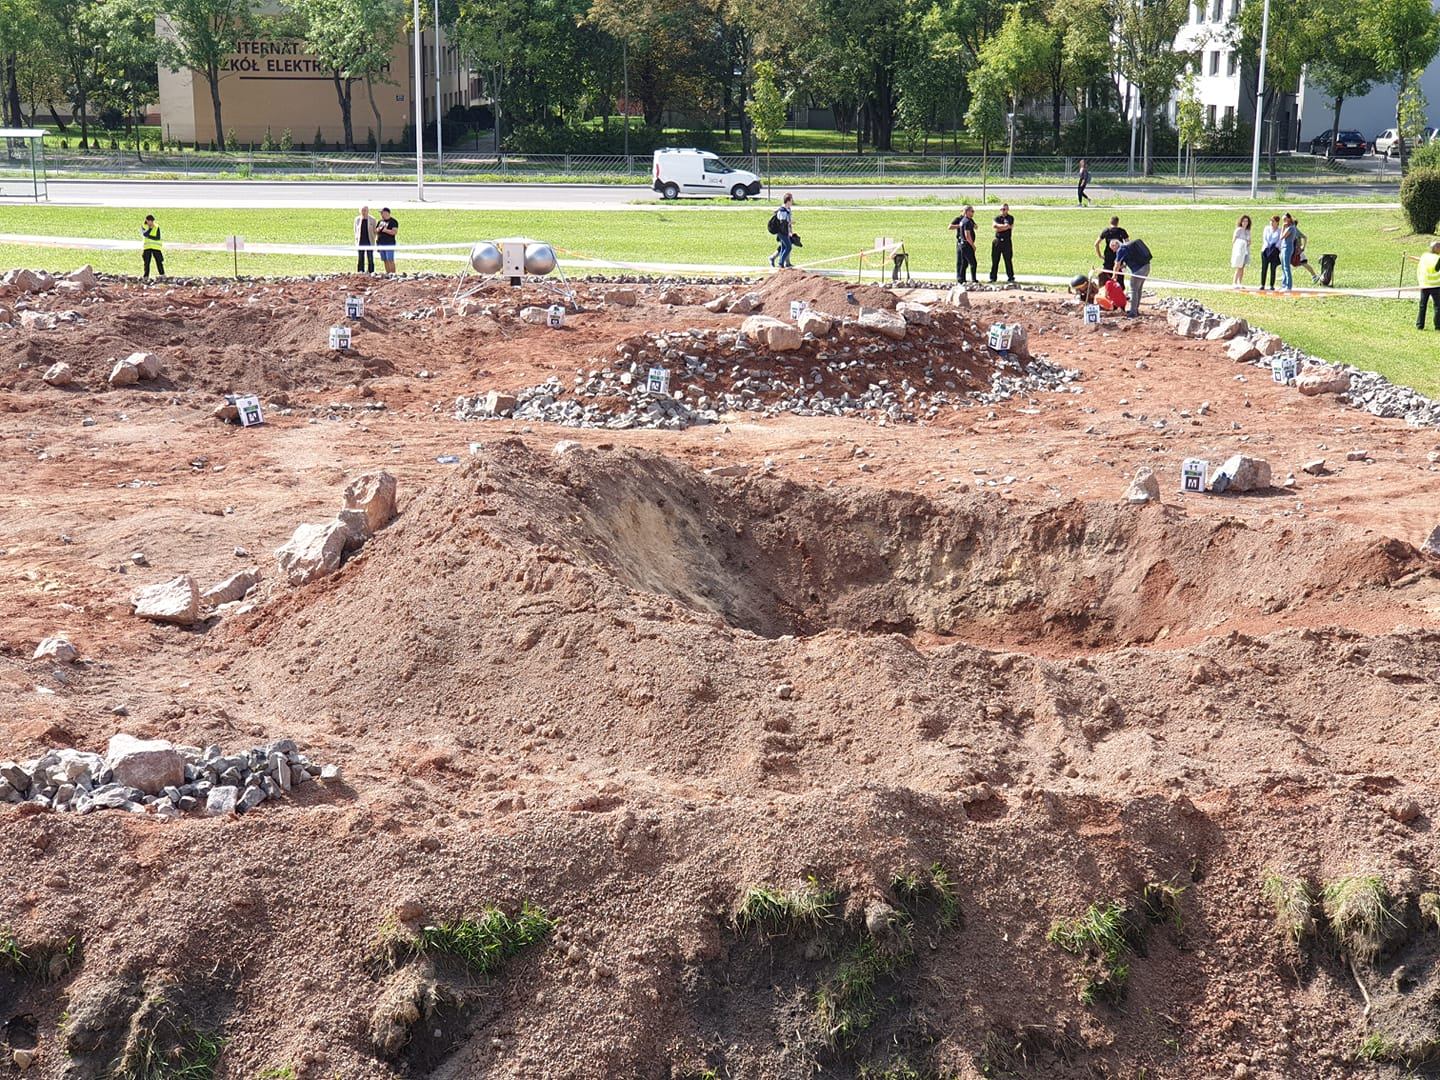
\includegraphics[width=0.6\textwidth]{image/terrain.jpeg}
		\caption{Terreno marziano a European Rover Challenge 2019}
		\label{fig:ercterrain}
	\end{figure}

	\section{Scenari affrontati nelle competizioni e ruolo di un manipolatore robotico}
		Le competizioni si svolgono su un terreno accidentato, realizzato da esperti di terrameccanica che vanno a simulare il più possibile uno scenario marziano. 
		Le task vengono svolte in un tempo limitato con il Robot teleoperato e gli operatori sono isolati dalla vista diretta all'interno di una control room. 
		
		L'unica task che non coinvolge l'uso del manipolatore robotico è quella di \textbf{Navigazione autonoma} che non tratteremo. 
		Pertanto segue l'analisi degli scenari di utilizzo. 
		\subsection{Manutenzione}
		La  maintanance task come definita dal regolamento 
		\textit{ERC 2019 Student Rules} \cite{ERC2019} 
		\newline
		\textit{The maintenance task is intended to demonstrate rovers and teams ability and performance in operating electrical panel on which several switches and other electrical components are mounted. The Team has to use rover’s manipulating device to set switches to correct positions, measure electrical parameters, set other panel controls and observe device feedback.}

		\newline
		\textbf{Successione di operazioni da svolgere :}
		\begin{enumerate}
		\item MAIN switch set to ON position as first;
		\item Group 1 and Group 2 switches set up to requested positions;
		\item knob set up to requested position
		\item voltage measurement reported to the judge
		\item High-power plug inserted into the sock
		\item No panel damage events occured (control elements, connectors, covers, foils
		\item task automation efforts and results presented to the judge.	 
		\end{enumerate}
	
		\begin{figure}
		\centering
		\begin{tabular}{ll}
		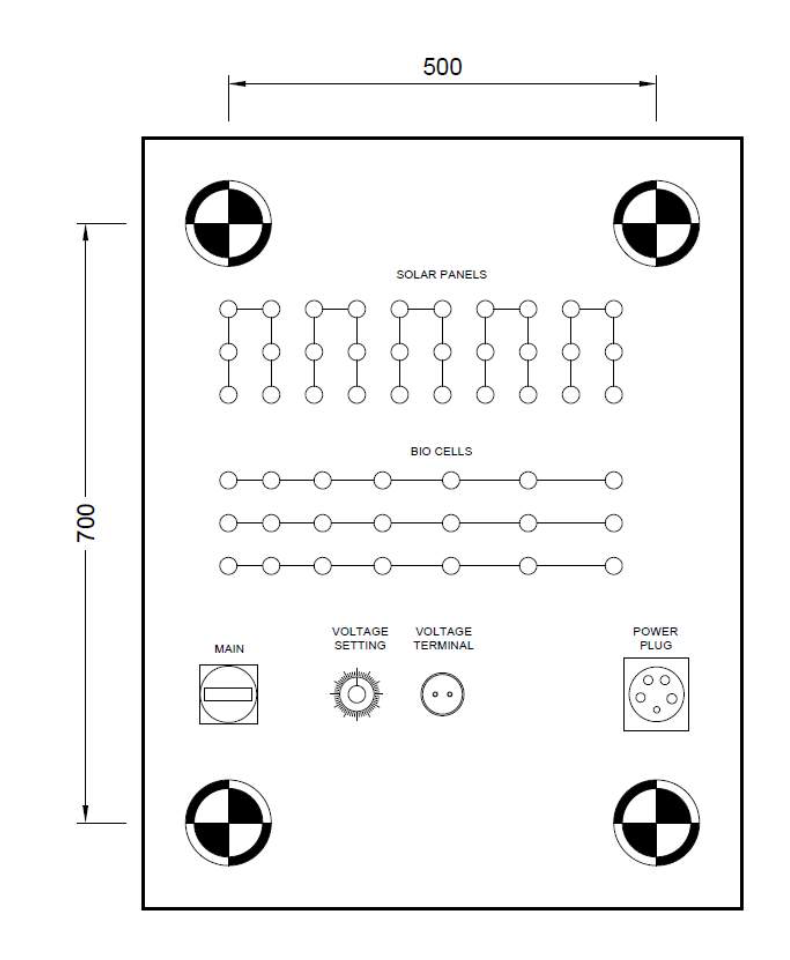
\includegraphics[width=0.4\textwidth]{image/panel.png}
		&
		\includegraphics[width=0.5\textwidth]{image/mainttoro.jpg}
		\end{tabular}
		\caption{Pannello Elettrico e Rover durante la Task}
		\label{fig:maintanance}
		\end{figure}
	
		\subsection{Raccolta di campioni scientifici}
		\subsection{Scenario Fetch and Collect}

\chapter{Analisi preliminare dei requisiti}
Ogni progetto di applicazione aerospaziale, come quello svolto per il Rover Trinity, parte dall'analisi dei requisiti di progetto e dalla formalizzazione dei requisiti in maniera codificata. 
La tracciabilità dei requisiti, analizzati a partire da uno scenario di missione e dalla vigente normativa è fondamentale all'interno di un progetto aerospaziale perchè consente di semplificare gli sviluppi futuri.
La costituzione di un database di requisiti, lezioni apprese e errori commessi nel caso in cui i requisiti vengano disattesi consente di abbattere i costi e le tempisitiche di sviluppo di progetti futuri evitando la ripetizione di esperimenti ed errori commessi in passato. 




	
	\renewcommand{\arraystretch}{1.2}
	\begin{longtable}{|p{0.10\textwidth}|p{0.27\textwidth}|p{0.27\textwidth}|p{0.27\textwidth}| } 
		\hline
		 \textbf{ORIG.}& \textbf{REQUISITO}& \textbf{SOLUZIONE     TECNICA}&  \textbf{VALIDAZIONE}\\*  &   &  &      \\* \hline
		\hline
	%ARM ASSUMPTION
		
	ERC &
	Il sottosistema braccio deve essere in grado di raggiungere il terreno, 
	raggiungere tutta la superficie dello chassis del rover, 
	raggiungere 1.5 metri di altezza, 
	manipolare elementi nello spazio tridimensionale &
	Manipolatore robotico antromorfo a 6 assi: dalla letteratura
	è la soluzione con la maggior destrezza	 & Modellazione CAD assieme allo chassis del Rover, Script di calcolo del workspace, modello multibody	\\*	&   &  &      \\* \hline
	
	
	ERC & 
	Il Sottosistema braccio deve essere in grado di sollevare almeno un payload di 5kg &
	Robot attuato da motoriduttori passo-passo, attuatori lineari e servomotori ad elevata coppia
	Trasmissione mediante riduttore a ruote dentate &
	CAD design del braccio, Matlab script del workspace, modello multibody, modello FEM, teoria di Lewis	\\*	&   &  &      \\* \hline
	
	MISSION & Il braccio deve avere elevata velocità operativa senza sacrificare l'accuratezza (target of tool center point of 1$cm^2$) & 
	Controllo in microstep dei motori passo passo, encoder relativo per attuatore lineare
	controllo in posizione dei servomotori &  
	Modello Simulink e cinematica inversa	\\*	&   &  &      \\* \hline

	MISSION & Il braccio deve essere in grado di raggiungere il pannello manutenzione posizionato a 0.5m di distanza 
	con il tool center point perpendicolare & 
	
	Polso Sferico & CAD design, Matlab script, multibody model \\*	&   &  &      \\* \hline
	
\caption{Tabella dei requisiti derivati dal progetto e dal regolamento}	
\end{longtable}
	\section{Workspace necessario}
	Il workspace richiesto per il manipolatore deriva dalle richieste del regolamento e dallo scenario operativo. Si può riassumere nella necessità di raggiungere un altezza di 1,5 metri e quella del suolo e operare sullo chassis del rover per depositare oggetti e campioni. 
	Il workspace è stato valutato attraverso un semplice calcolo iterativo di cinematica diretta dove la struttura era parametrizzata attraverso le lunghezze dei link. L'obiettivo è quello di realizzare uno spazio di lavoro sufficiente plottando la posizione dell Tool Center Point per ogni iterazione in una vista laterale. 
	Una volta decise delle lunghezze dei link principali è stato possibile iniziare la costruzione dei primi modelli cad della struttura del robot per poterne costruire un modello dinamico e non solo più cinematico. 
	
	
	\begin{figure}
		\centering
		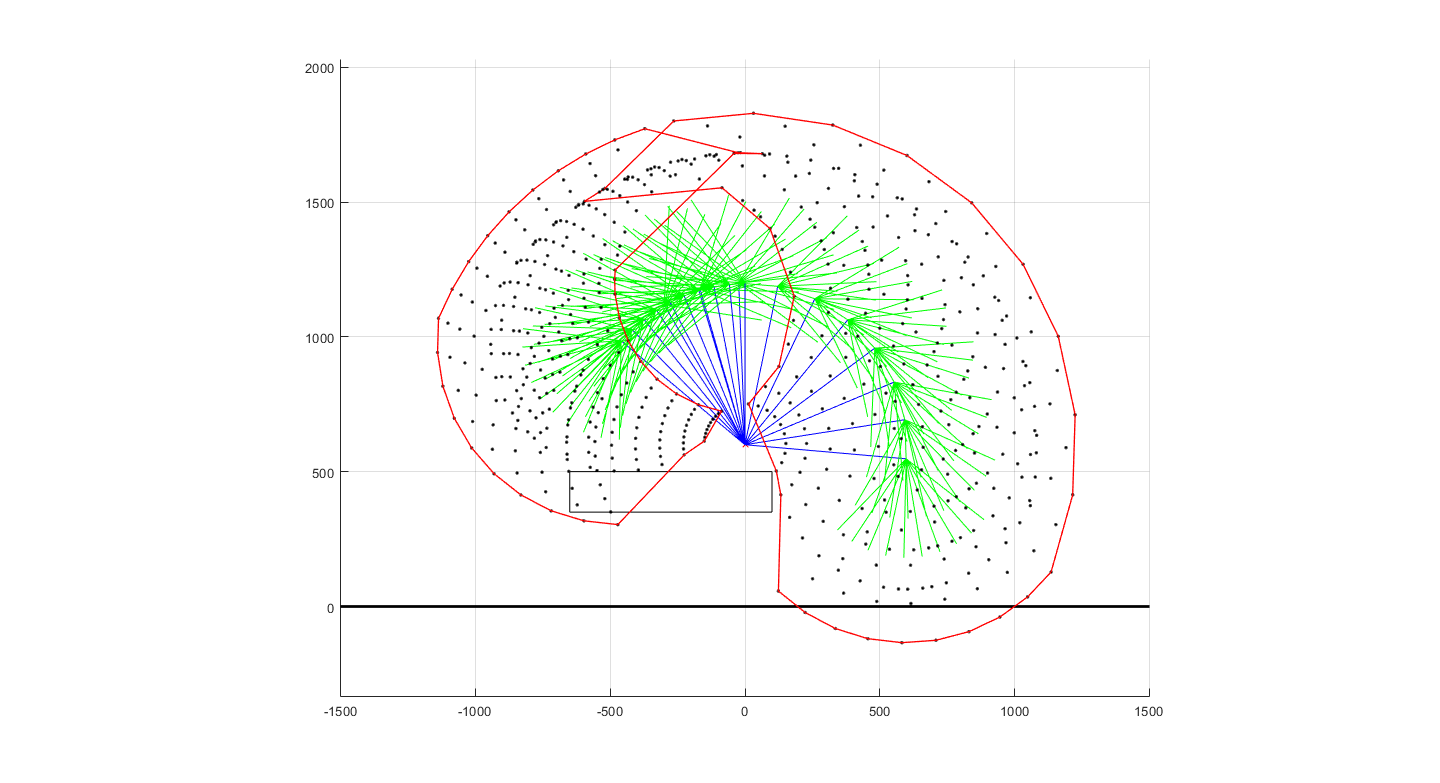
\includegraphics[width=\textwidth]{Plots/workspace.png}
		\caption{Workspace in vista laterale, è rappresentato il piano dello chassis e i punti raggiunti dal TCP}
		\label{fig:workspace}
	\end{figure}
	
	\section{Gradi di libertà necessari}
	\section{Task di manipolazione e destrezza: Worst case}

\chapter{Design di un manipolatore a 6 gradi di libertà}
\section{Descrizione del modello di Robot}
La configurazione scelta è quella di un manipolatore antropomorfo a 6 assi. La struttura per i primi tre assi è realizzata tramite link in profilati di alluminio estrusi e parti lavorate sempre in alluminio mentre le cerniere sono realizzate da alberi in acciaio supportati da boccole a basso coefficiente di attrito. I rimanenti tre assi sono collocati nel Polso Sferico all'estremità, un componente in manifattura additiva che verrà trattato più ampiamente in seguito. 
	\begin{figure}
	\centering
	\includegraphics[width=0.7\textwidth]{pictures/ARM.png}
	\caption{Render del modello CAD preliminare del robot}
	\label{fig:render}
\end{figure}
	\begin{figure}
	\centering
	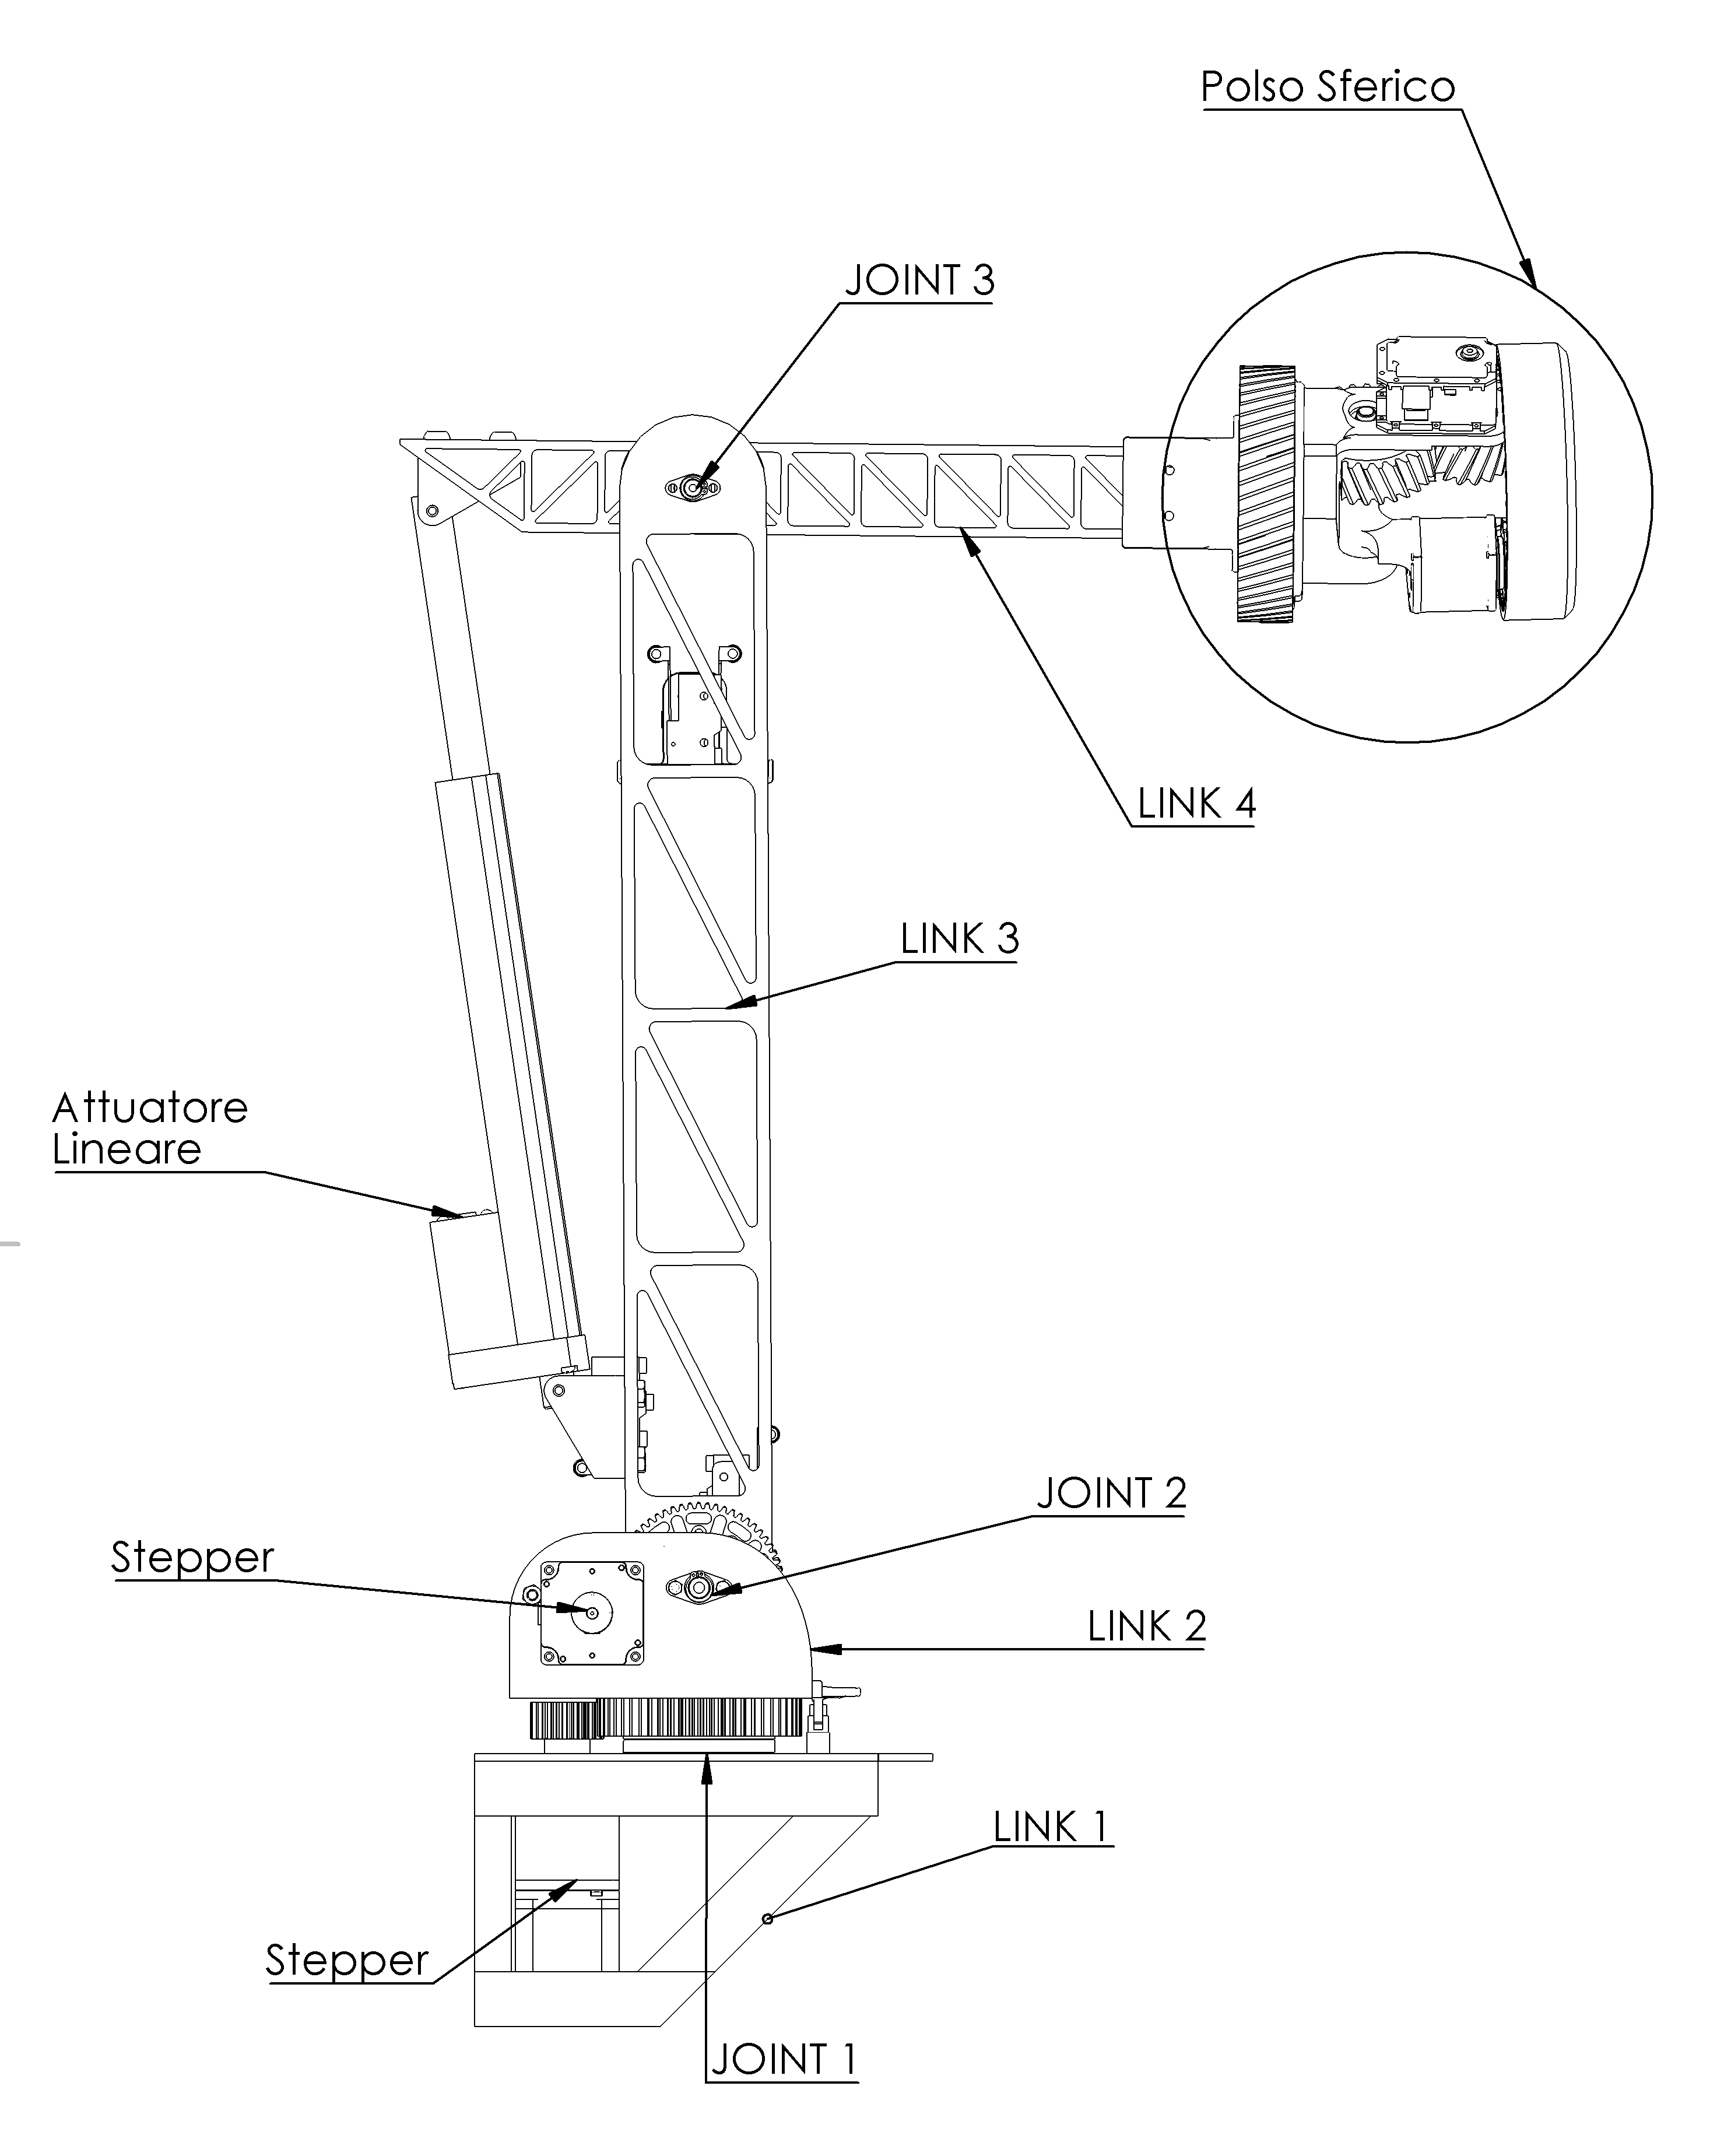
\includegraphics[width=0.7\textwidth]{Screen/ARMBollato.png}
	\caption{Schema delle componenti}
	\label{fig:bollatura}
\end{figure}
Il robot è schematizzato nel disegno \ref{fig:bollatura} e nel capitolo 4 verrà analizzato il dimensionamento degli attuatori \textit{Stepper} e dell'\textit{Attuatore Lineare} mentre al \textbf{Polso Sferico} sarà dedicato il capitolo 5. 

	
	\section{Modello multibody}
	La costruzione di un modello multibody del robot è fondamentale per avere uno strumento di analisi delle prestazioni richieste agli attuatori e poter selezionare dei componenti adatti sul mercato. 
	Per l'analisi della dinamica del robot è stato costruito un modello multibody attraverso il software \textit{MSC Adams}. \\
	Un sistema dinamico multibody consiste di corpi solidi connessi tra loro tramite giunti che ne limitano o impongono il relativo movimento. Lo studio della dinamica multibody è l’analisi di come questi sistemi si muovono sotto l’influenza di specifiche forze, detta anche dinamica diretta. Lo studio del problema opposto, cioè di quali forze sono necessarie a far muovere il sistema meccanico in un modo specifico è detta dinamica inversa.\\
	La possibilità di studio della dinamica inversa ha permesso di studiare le prestazioni richieste agli attuatori del robot e dimensionare di conseguenza i componenti meccanici della trasmissione. 
	Eseguita la simulazione è possibile raccogliere le misure richieste e processare i dati raccolti nello strumento di raccolta dati \textit{Adams/PostProcessor}. 
		\begin{figure}
		\centering
		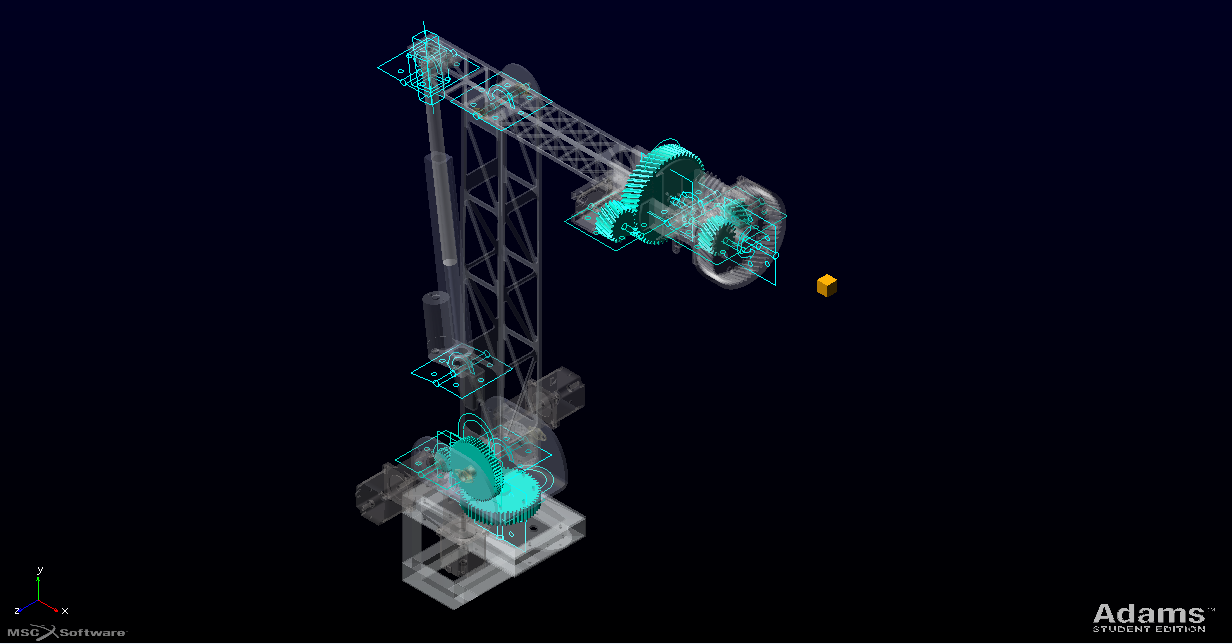
\includegraphics[width=\textwidth]{Screen/Model1.png}
		\caption{Modello del Robot in ambiente Adams, in ciano le icone dei giunti e le trasmissioni mediante ruote dentate}
		\label{fig:adamsmodel}
	\end{figure}
	
	Il modello del robot \ref{fig:adamsmodel} è stato costruito a partire dal modello CAD preliminare \ref{fig:render} modellato in ambiente \textit{SolidWorks} importato nello spazio di lavoro di \textit{Adams/View}. I singoli componenti sono stati dotati delle relative matrici di inerzia riferite a un sistema di riferimento favorevole al calcolo dall'output di proprietà di massa del CAD e riferite ad un analogo \textit{Marker} del modello di simulazione. Così facendo la simulazione permetterà di calcolare le forze necessarie affinchè si rispettino le leggi di moto imposte ai giunti.
			\begin{figure}
			\centering
			\begin{tabular} {ll}
		
			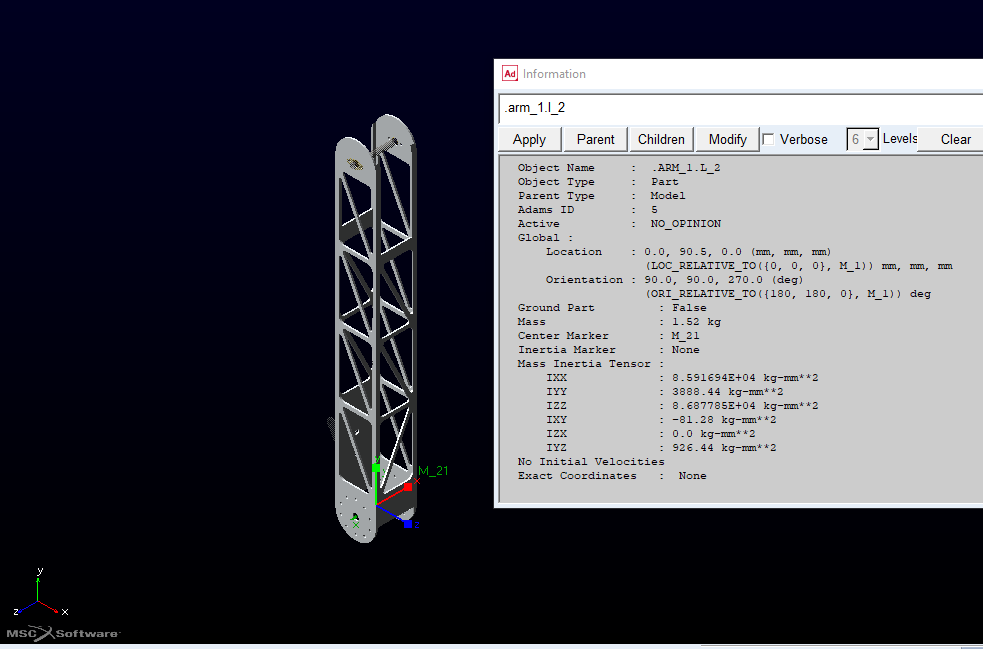
\includegraphics[width=0.5\textwidth]{Screen/inertia.png}
			&
			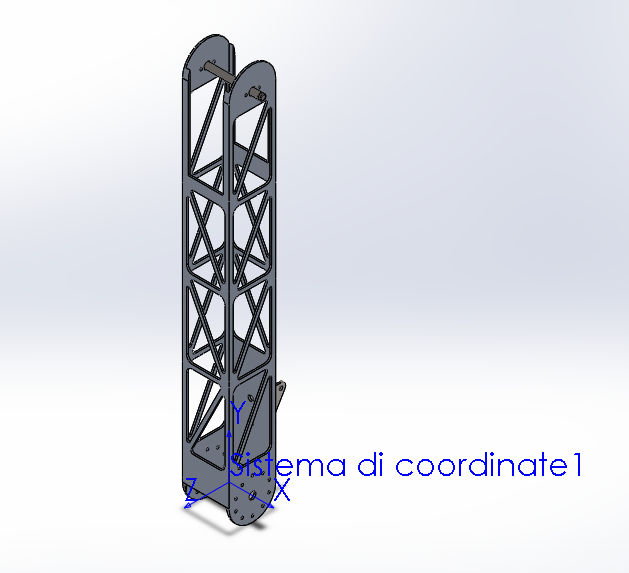
\includegraphics[width=0.4\textwidth]{Screen/coordinate.png}
			\end{tabular}
			\caption{Proprietà inerziali del componente e sistema di coordinate nel CAD}
			\label{fig:inertia}
			\end{figure}
	 Inoltre il modulo \textit{Adams/Machinery} consente di modellare trasmissioni mediante accoppiamento di ruote dentate e di simularne il comportamento con vari livelli di approssimazione. Nella fattispecie si è scelto l'approccio semplificato che studia il problema di contatto mediante metodo analitico monodimensionale, in modo da fornire un confronto e una verifica del dimensionamento realizzato. 
	
	
	
	
	
	
		

\chapter{Attuatori per un progetto di robotica low-cost} \label{attuatori}
	\section{Motoriduttori Passo-Passo, trasmissione del Moto e componenti utilizzati}
		\subsection{Joint 1}
		\subsection{Joint 2}
		\subsection{Cenni di controllo ad anello aperto}
	\section{Attuatori Lineari, Cinematismo Joint 3}
		
	\section{Servomotori digitali: Dynamixel MX160}
		\subsection{Scelta ed integrazione, i vantaggi di un attuatore specifico per impiego robotico}
		
\chapter{Polso sferico, design e scelte progettuali}
	\section{Descrizione}
	\section{Ingombri ed integrazione}
	\section{Scelta dei Cuscinetti}
	\section{Metodo di Lewis}
	\section{Riduzione del numero minimo di denti: ingranamento elicoidale}
	\section{Dimensionamento di un rotismo stampato in 3D, compromessi e assunzioni}
	\section{Risultati ottenuti dal dimensionamento}
	\section{Compromesso tra dimensionamento e ingombri}

\chapter{Costruzione mediante manifattura additiva e assemblaggio}
	\section{Studio del materiale da stampa ABSPlus P430}
	\section{Produzione dei componenti}
	\section{Assemblaggio}
\chapter{Risultati attesi ed ottenuti dal Robot realizzato}
	\section{Test e collaudo del Robot assemblato}
	\section{Carichi massimi applicati e precisione ottenuta}
	\section{Risultati nelle Competizioni studentesche }

\backmatter
\chapter{Disegni ed elaborati tecnici}







\begin{thebibliography}{9}
\bibitem{ERC2019} European Rover Challenge, \emph{Student Rules}, ERC, gennaio 2019

\bibitem{tor1} E.~Torricelli, in ``La pressione barometrica'', {\em Strumenti
        Moderni}, Il Porcellino, Firenze, 1606.
\bibitem{tor2} E.~Torricelli e A.~Vasari, in ``Delle misure'', {\em Atti Nuovo
        Cimento}, vol.~III, n.~2 (feb. 1607), p.~27--31.
\bibitem{duane1964} Duane J.T., \emph{Learning Curve Approach To Reliability 
		Monitoring}, IEEE Transactions on Aerospace, Vol. 2, pp. 563-566, 1964
\end{thebibliography}

\end{document}

% altri riferimenti da usare come esempi.

\bibitem{ERC2019} European Rover Challenge, \emph{Student Rules}, ERC, gennaio 2019
	
	
\bibitem{chiesa2}Chiesa S., Fioriti M., Fusaro R., \emph{On Board System 
		Technological  Level Improvement Effect on UAV MALE}
\bibitem{bigliano2010} Bigliano M., \emph{Sicurezza nell'installazione di un velivolo 
		senza pilota MALE; applicazione di metodologia di Zonal Safety 
		Analysis al velivolo del Progetto SAvE}, Politecnico di Torino, 
		maggio 2010
\bibitem{astrid2012} Chiesa S., Di Meo G.A., Fioriti M., Medici G., Viola N.,
		\emph{ASTRID - Aircraft on board Systems sizing and TRade-off 
		analysis in Initial Design}, Research Bulletin, Warsaw University 
		of Technology, Institute of Aeronautics and Applied Mechanics, 
		p. 1-28, 17-19, ottobre 2012

